\chapter{Results}
For RQ1, our study has shown a way of analyzing conflict resolutions in large-scale codebases, and this can be achieved by parsing output from Conflicts Analyzer. Likewise, for RQ2, we have created a categorization for merge-conflicts resolved by developers which can be used in future studies to, for instance, create an automatic merge tool. This chapter shows the results of the manual- and automatic analysis.
\section{Manual Analysis}
For conflicts in the conflict pattern SameSignatureCM, we found that if one of the two versions had the same code as the other version but with some additional code, that version was often chosen as resolution. This can be seen in Table \ref{table:rcsitma} where the resolution was a superset in 69\% of the cases. Table \ref{table:rcsitma} lists how many resolutions, in the 26 cases that were analyzed, were \textit{Superset}, \textit{Intersection} and/or \textit{Recent}. As a resolution can be both recent and a superset or an intersection at the same time, the percentage add up to more than 100\%.
\begin{table}
\caption{Results of the manual analysis for the properties in Table \ref{table:pproperties}}\label{table:rcsitma}
\begin{tabular}{ p{6cm} p{6cm} }
\hline
\multicolumn{1}{c}{\textbf{Property}} & \multicolumn{1}{c}{\textbf{Number of cases (total 26 cases)}}\\
Superset & 18 (~69\%)\\
Recent & 15 (~58\%)\\
Intersection & 4 (~15\%)\\
\end{tabular}
\end{table}
\FloatBarrier
For some of the cases that were chosen as resolution, one or more if-statements had been introduced in the version that was chosen which the other version did not have. We also saw an example of a case where the chosen version had more error handling than the other version.

An example can be seen from the repository Android-async-http, where two versions that resulted in a conflict when being merged looked like this:\\
\textbf{Left version:}
\lstset{language=Java,numbers=left,xleftmargin=2em,frame=single,framexleftmargin=1.5em}
\begin{lstlisting}[frame=single,breaklines=true,tabsize=2]
protected void sendSuccessMessage(int statusCode, Header[] headers, String responseBody) {
	try {
		Object jsonResponse = parseResponse(responseBody);
		sendMessage(obtainMessage(SUCCESS_JSON_MESSAGE, new Object[]{statusCode, headers, jsonResponse}));
	} catch(JSONException e) {
		sendFailureMessage(e, responseBody);
	}
}
\end{lstlisting}
\textbf{Right version:}
\lstset{language=Java,numbers=left,xleftmargin=2em,frame=single,framexleftmargin=1.5em}
\begin{lstlisting}[frame=single,breaklines=true,tabsize=2]
protected void sendSuccessMessage(int statusCode, Header[] headers, String responseBody) {
	if (statusCode != HttpStatus.SC_NO_CONTENT){
		try {
			Object jsonResponse = parseResponse(responseBody);
			sendMessage(obtainMessage(SUCCESS_JSON_MESSAGE, new Object[]{statusCode, headers, jsonResponse}));
		} catch(JSONException e) {
			sendFailureMessage(e, responseBody);
		}
	} else {
		sendMessage(obtainMessage(SUCCESS_JSON_MESSAGE, new Object[]{statusCode, new JSONObject()}));
	}
}
\end{lstlisting}
Here, all the words in the left version are also in the right version, hence the right is a superset of the left version. In this example, the right version was chosen as the resolution. As can also be seen, in the right version there is a check by an if-statement that is not present in the left version.
\FloatBarrier
\section{Automatic Analysis}
\FloatBarrier
The automatic analysis that was conducted on the 20 top starred Java projects on GitHub yielded, after our filtering, 1964 conflicts. For each property (see Table \ref{table:propdef}), the resolutions for the 1964 conflicts was categorized according to Table \ref{table:pproperties2} and the results are presented in this section.
\subsection{Developers often choose one version completely}
\FloatBarrier
In 1509 cases (77\% of the studied cases), the left version was chosen as resolution, that is, the version that was checked out at the time of merging. Figure \ref{fig:groups} shows how many cases where the left- and right version was chosen completely as the resolution and in how many cases none of them were chosen completely.

\begin{figure}
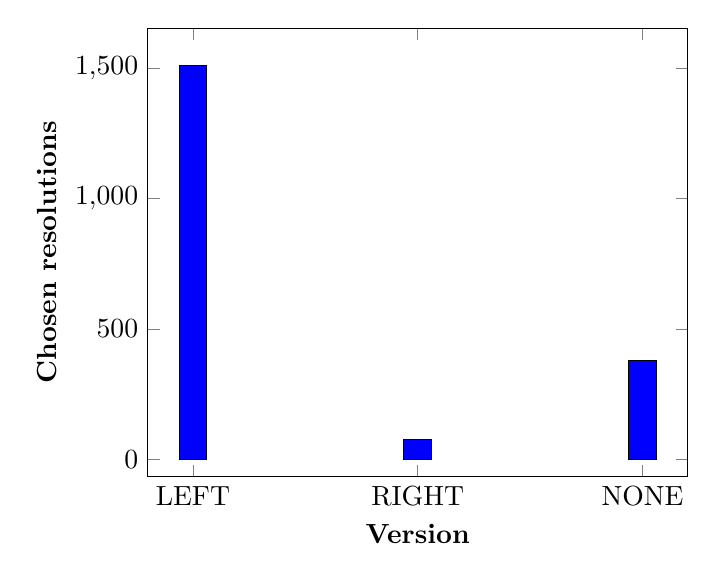
\begin{tikzpicture}
\begin{axis}[
   symbolic x coords={LEFT, RIGHT, NONE},
   xtick=data,
   xlabel=\textbf{Version},
   ylabel=\textbf{Chosen resolutions}
 ]
   \addplot[ybar,fill=blue] coordinates {
       (LEFT,   1509)
       (RIGHT,  77)
       (NONE,   378)
   };
\end{axis}
\end{tikzpicture}
\caption{Number of chosen resolutions}\label{fig:groups}
\end{figure}
\FloatBarrier

%Total:
%TOT: flest,		färst, 		ingen, Non applicable
%	 recent, 	not recent		 , Non applicable
%	 sup/int	den andra	none , Non applicable

\subsection{Properties}
Figure \ref{set} shows the resolution categorization, as defined in Table \ref{table:pproperties2} for each property, as defined in Table \ref{table:propdef}. The figure shows that the chosen version often is the more recent. It also shows that if one of the versions is a superset of the other, the version that is the superset is often chosen. On the contrary, if one version is an intersection of the two versions, the other version is more often chosen. For the if-statements, print-instances, log-instances and try-instances there were too many resolutions in the Not applicable category to draw any conclusions.

Figure \ref{setleft} shows the resolution categorization where X is the left version and Y is the right version, and Figure \ref{setright} shows the resolution categorizations where X is the right version and Y is the left version. From these figures, one can see that the left version more often is a superset of the right version than the other way around. On the contrary, the right version
\FloatBarrier
\begin{figure}
\resizebox {\columnwidth} {!} {
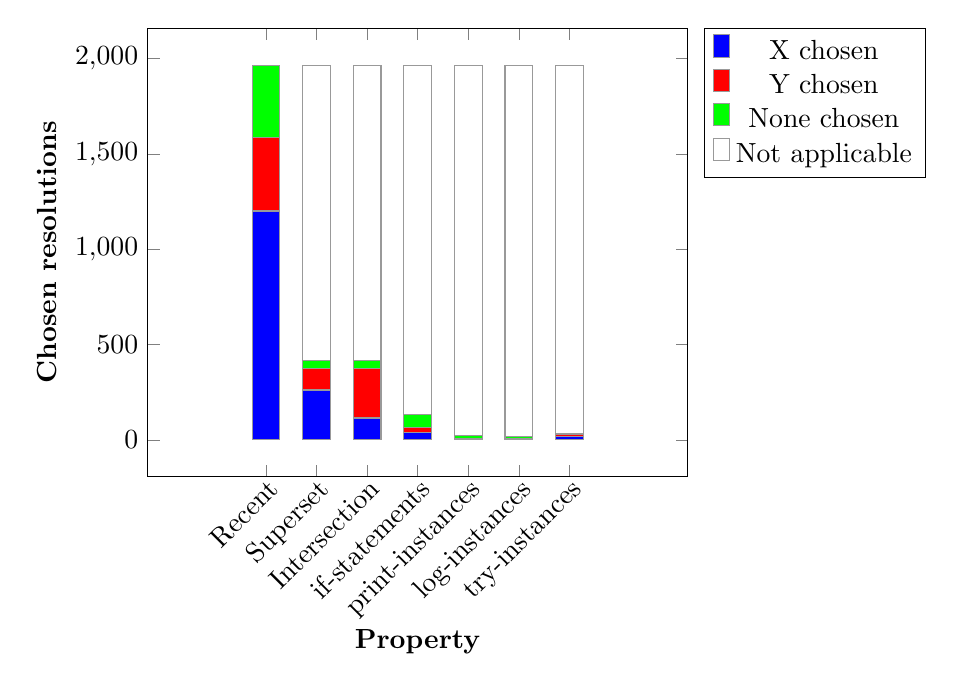
\begin{tikzpicture}
\begin{axis}[ybar stacked,symbolic x coords={Recent,Superset,Intersection,if-statements,print-instances,log-instances,try-instances},xtick=data,enlarge x limits={abs=1.5cm},xlabel=\textbf{Property},ylabel=\textbf{Chosen resolutions},legend pos=outer north east,
 xticklabel style={
         inner sep=0pt,
         anchor=north east,
         rotate=45 }
 ]
]
  \addplot[black!40,fill=blue] coordinates{(Recent,1201)(Superset,262)(Intersection,115)(if-statements,39)(print-instances,6)(log-instances,4)(try-instances,17)};
  \addplot[black!40,fill=red] coordinates{(Recent,385)(Superset,115)(Intersection,262)(if-statements,26)(print-instances,2)(log-instances,5)(try-instances,11)};
  \addplot[black!40,fill=green] coordinates{(Recent,378)(Superset,42)(Intersection,42)(if-statements,67)(print-instances,13)(log-instances,7)(try-instances,7)};
  \addplot[black!40,fill=white] coordinates{(Recent,0)(Superset,1545)(Intersection,1545)(if-statements,1832)(print-instances,1943)(log-instances,1948)(try-instances,1929)};
\legend{X chosen, Y chosen, None chosen, Not applicable}
\end{axis}
\end{tikzpicture}
}
\caption{Resolution categorization for each property.}\label{set}
\end{figure}

\begin{figure}
\resizebox {\columnwidth} {!} {
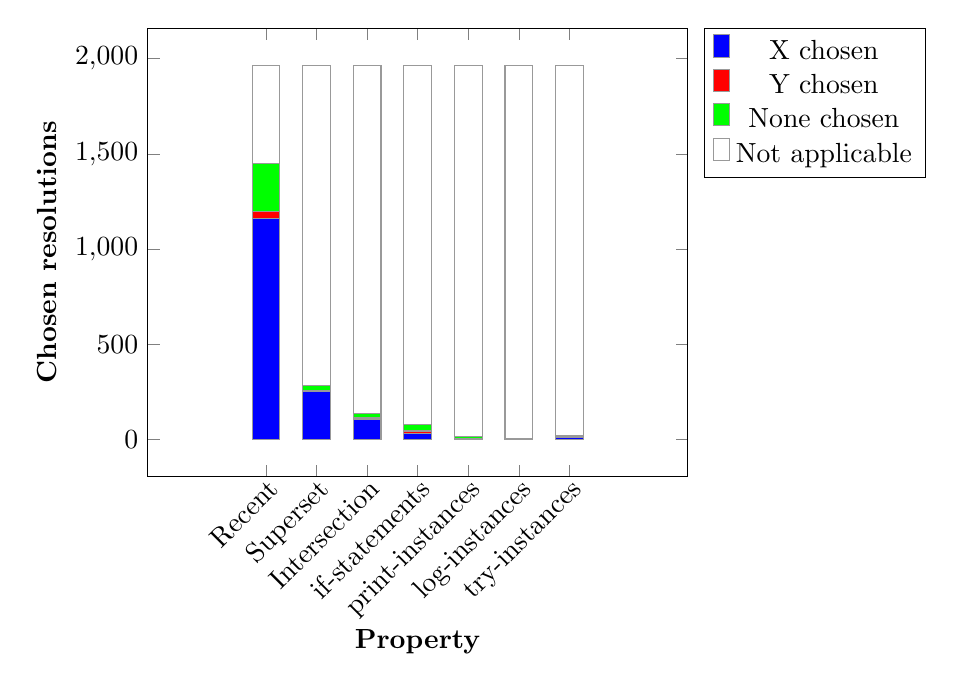
\begin{tikzpicture}
\begin{axis}[ybar stacked,symbolic x coords={Recent,Superset,Intersection,if-statements,print-instances,log-instances,try-instances},xtick=data,enlarge x limits={abs=1.5cm},xlabel=\textbf{Property},ylabel=\textbf{Chosen resolutions},legend pos=outer north east,
xticklabel style={
         inner sep=0pt,
         anchor=north east,
         rotate=45 }]
  \addplot[black!40,fill=blue] coordinates{(Recent,1161)(Superset,253)(Intersection,108)(if-statements,32)(print-instances,6)(log-instances,2)(try-instances,13)};
  \addplot[black!40,fill=red] coordinates{(Recent,37)(Superset,7)(Intersection,9)(if-statements,13)(print-instances,0)(log-instances,0)(try-instances,4)};
  \addplot[black!40,fill=green] coordinates{(Recent,252)(Superset,22)(Intersection,20)(if-statements,32)(print-instances,10)(log-instances,5)(try-instances,4)};
  \addplot[black!40,fill=white] coordinates{(Recent,514)(Superset,1682)(Intersection,1827)(if-statements,1887)(print-instances,1948)(log-instances,1957)(try-instances,1943)};
\legend{X chosen, Y chosen, None chosen, Not applicable}
\end{axis}
\end{tikzpicture}
}
\caption{Resolution categorization for each property, where X is the left version and Y is the right version.}\label{setleft}
\end{figure}

\begin{figure}
\resizebox {\columnwidth} {!} {
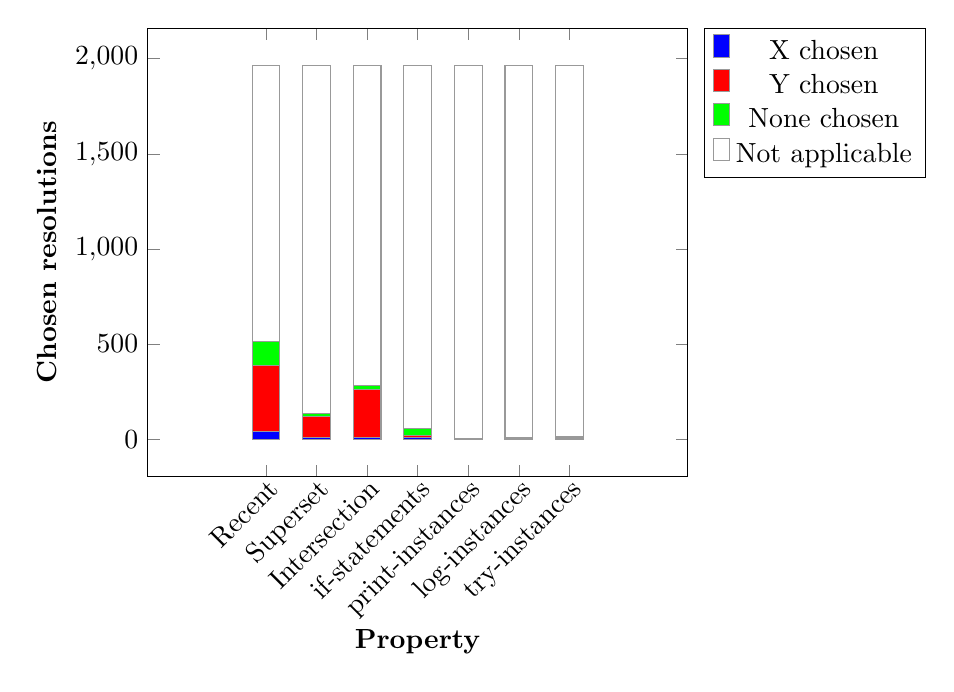
\begin{tikzpicture}
\begin{axis}[ybar stacked,symbolic x coords={Recent,Superset,Intersection,if-statements,print-instances,log-instances,try-instances},xtick=data,enlarge x limits={abs=1.5cm},xlabel=\textbf{Property},ylabel=\textbf{Chosen resolutions},legend pos=outer north east,
xticklabel style={
         inner sep=0pt,
         anchor=north east,
         rotate=45 }]
  \addplot[black!40,fill=blue] coordinates{(Recent,40)(Superset,9)(Intersection,7)(if-statements,7)(print-instances,0)(log-instances,2)(try-instances,4)};
  \addplot[black!40,fill=red] coordinates{(Recent,348)(Superset,108)(Intersection,253)(if-statements,13)(print-instances,2)(log-instances,5)(try-instances,7)};
  \addplot[black!40,fill=green] coordinates{(Recent,126)(Superset,20)(Intersection,22)(if-statements,35)(print-instances,3)(log-instances,2)(try-instances,3)};
  \addplot[black!40,fill=white] coordinates{(Recent,1450)(Superset,1827)(Intersection,1682)(if-statements,1909)(print-instances,1959)(log-instances,1955)(try-instances,1950)};
\legend{X chosen, Y chosen, None chosen, Not applicable}
\end{axis}
\end{tikzpicture}
}
\caption{Resolution categorization for each property, where X is the right version and Y is the left version.}\label{setright}
\end{figure}
\FloatBarrier
\section{Discussion}
The most significant result in this study is that in cases of conflicting code in methods or constructors, in 3 out of 4 cases that we studied, developers chose the left version when merging. The reasons for this is unclear, but there are two main scenarios; when pulling a remote branch and when merging a local branch into another one.

The left version is the commit that the developer who performs the merge has checked out when merging. If the conflicting merge is a result of pulling a remote branch, the left version is likely his own code, and the right version is someone else’s code. Figure \ref{set} shows that the chosen version also often is the most recent version. This in combination with that the left version most often is chosen indicates that developers tend to choose their own code as resolution. This study has not gone into why developers resolve conflicts this way, but it might be interesting for future studies to investigate this further. If the conflicting merge is a result of merging a local branch into another one, the left version is the branch which the other branch was merged into.

\subsection{Threats to Validity}
\subsubsection{Construct Validity}
Although the tools used throughout the study, Conflicts Analyzer and Resolutions Analyzer, have been developed with great care, there is still the risk of the tools containing bugs which might lead to an inaccurate result.
\subsubsection{External Validity}
Our results are based on a sample of 20 projects of different sizes, and a total of 1964 conflicts were analyzed. The results might differ if other projects were to be analyzed. The 20 top starred projects were all Java projects. Thus we can not say if our results hold for other languages. Also, these were all open-source projects and may not hold for closed-source projects. The fact that the projects are the 20 most top starred projects on Github might also affect the results.
\subsubsection{Conclusion Validity}
To show that the results are not random, we have done a statistical analysis on the results using Chi squared tests. We tested the results to show that they are significant. The Chi squared tests was conducted on the results, see Figure \ref{set}, for each property, see Table \ref{table:propdef}. The expected values are here calculated by dividing the total amount of cases in the categories X chosen and Y chosen by 2. Thus, cases in the categories None chosen and Not applicable are not included in the Chi squared tests and therefore, the total number of cases in the X chosen and Y chosen categories will differ depending on the property. We also conducted a Chi square test on the result for Left and Right versions chosen, see Figure \ref{fig:groups}. The expected values are here calculated by dividing the total amount of cases where one version was chosen completely by 2. The tested hypotheses are defined in Table \ref{table:hypotheses}. We reject H\textsubscript{0} if the p value is lower than 0.05. With a degree of freedom of 1, the required Chi square is 3.84. The Chi square results are shown in Table \ref{table:pchi} and Table \ref{table:vchi}. Note that for the properties print-instances and log-instances, the expected values are lower than 5, which is a limitation for the Chi square test and we do not draw any conclusions about those properties.

\begin{table}[htbp]
\caption{Hypotheses}
\label{table:hypotheses}
\begin{tabular}{|l|p{6cm}|p{6cm}|}
\hline
& \textbf{H\textsubscript{0}} & \textbf{H\textsubscript{a}}\\
\hline
\textbf{Properties} & When a property is satisfied and either X or Y was chosen as resolution, the property does not affect what version developers choose when resolving conflicts. & When a property is satisfied and either X or Y was chosen as resolution, the property affects what version developers choose when resolving conflicts.\\
\hline
\textbf{Chosen versions} & Whether a version is Left or Right does not affect which of the versions developers choose when resolving conflicts. & Whether a version is Left or Right affects which of the versions developers choose when resolving conflicts.\\
\hline
\end{tabular}
\end{table}

\begin{table}[htbp]
\caption{Chi square tests for the properties}
\label{table:pchi}
\begin{tabular}{|l|l|l|l|l|l|l|l|}
\hline
\centering \textbf{Property} & \multicolumn{2}{c|}{\centering \textbf{X chosen}}& \multicolumn{2}{c|}{\centering \textbf{Y chosen}}&\multirow{2}{*}{\textbf{Total}}&\multirow{2}{*}{\makecell{\textbf{Chi}\\ \textbf{square}}}&\multirow{2}{*}{\makecell{\textbf{Reject}\\ \textbf{H\textsubscript{0}}}}\\
\cline{2-5}
& \textbf{Observed} & \textbf{Expected} & \textbf{Observed} & \textbf{Expected} & & & \\ \hline
Recent & 1201 & 793 & 385 & 793 & 1586 & 419.8 & Yes\\
Superset & 262 & 188.5 & 115 & 188.5 & 377 & 57.32 & Yes\\
Intersection & 115 & 188.5 & 262 & 188.5 & 377 & 57.32 & Yes\\
if-statements & 39 & 32.5 & 26 & 32.5 & 65 & 2.600 & No\\
print-instances & 6 & 4 & 2 & 4 & 8 & 2.000 & No\\
log-instances & 4 & 4.5 & 5 & 4.5 & 9 & 0.111 & No\\
try-instances & 17 & 14 & 11 & 14 & 28 & 1.286 & No\\
\hline
\end{tabular}
\end{table}

\begin{table}[htbp]
\caption{Chi square test for the chosen versions}
\label{table:vchi}
\begin{tabular}{|l|l|l|l|l|l|l|l|}
\hline
\multicolumn{2}{|c|}{\centering \textbf{Left}}& \multicolumn{2}{c|}{\centering \textbf{Right}}&\multirow{2}{*}{\textbf{Total}}&\multirow{2}{*}{\textbf{Chi square}}&\multirow{2}{*}{\textbf{Reject H\textsubscript{0}}}\\
\cline{1-4}
\textbf{Observed} & \textbf{Expected} & \textbf{Observed} & \textbf{Expected} & & & \\ \hline
1509 & 793 & 77 & 793 & 1586 & 1293 & Yes\\
\hline
\end{tabular}
\end{table}


